\chapter{Ionic Bonds: What Happens After Electron Transfer}

\begin{kaichang}
Find some table salt in the kitchen, sprinkle a little on white paper, and examine it with a magnifying glass---or take a close-up photo with your phone. The grains are not rounded like sand, but tiny, sharply edged square crystals, like miniature dice. Choose a larger grain, gently crush it with a hammer on the paper, and inspect the fragments: still square, only smaller.

Now make three guesses. First: why is salt so ``square''? Who prescribed such a neat shape? Second: salt vanishes almost instantly in water, yet sprinkled into a stove flame it merely turns the flame yellow (sodium's flame color from Chapter 9) and stubbornly refuses to melt. Why does it fear water but not fire? Third: dry salt does not conduct electricity at all, but dissolve that same spoonful in water and the solution conducts. There is no more or less salt. What changed?

Write down your three guesses. By the end of this chapter, we will check them against the astonishingly orderly ``city'' inside a salt grain.
\end{kaichang}

\section{Getting to Know Salt's Personality}

Before experimenting, let us line up the visible facts. Compare a small spoonful of salt with one of sugar, feature by feature, and you find intriguing differences:

\begin{itemize}[itemsep=2pt]
\item \textbf{Shape}: salt forms tiny cubes; sugar grains also have edges, but their crushed fragments are irregular.
\item \textbf{Hardness}: neither can be crushed between your fingers; both are quite hard.
\item \textbf{Impact resistance}: a hammer breaks sugar into irregular shards, but salt splits into neat little blocks, as though along invisible seams.
\item \textbf{Fire resistance}: heated above a hundred degrees Celsius, sugar melts, yellows, and chars. Salt heated over an ordinary flame for a long time merely glows red, otherwise unchanged: pure salt does not melt until $801\,^{\circ}\mathrm{C}$.
\item \textbf{Affinity for water}: both dissolve readily and are insulators when dry, yet their aqueous solutions behave very differently. Keep this in mind for the experiment later.
\end{itemize}

Two kinds of small white grains, with different personalities at every turn. Sugar's melting and charring belong to another kind of bonding (Chapter 19). Here we focus on salt: its squareness, brittleness, fire resistance, and changed conductivity ``before and after entering water'' all point to one explanation. Salt is not a collection of ``molecules,'' but a \textbf{vast arrangement of charged particles}.

\section{After the Handover: Two Ions Are Born}

Let us zoom inside a salt grain and see where its two kinds of particles come from. Earlier chapters have already rehearsed this scene:

A sodium atom has 11 electrons, arranged on floors as 2, 8, 1. The lone outer electron is far from the nucleus and heavily shielded by inner electrons, so it is easily pulled away. (Chapter 12 explained that this underlies sodium metal's violent reaction with water.) A chlorine atom has 17 electrons, arranged 2, 8, 7. Its outer floor is one electron short of full, and its nucleus has a strong grip, making chlorine a renowned electron snatcher (Chapter 13). On Chapter 11's scoreboard, sodium's electronegativity is only about 0.9, while chlorine's is about 3.2---a huge gap.

When these atoms meet, the outcome seems inevitable: chlorine takes sodium's outer electron completely. Sodium becomes a sodium ion with one positive charge and shells contracted to 2, 8; chlorine becomes a chloride ion with one negative charge and a completed 2, 8, 8 arrangement.

A fair trade, with everyone happy? Not so fast. Chapter 17 established that every change must balance its energy accounts. Separate this transaction into steps and its first half actually \textbf{loses money}: pulling an electron from sodium requires energy (ionization energy, Chapter 11), while delivering it to chlorine returns some energy (electron affinity), but not the full payment. If the story ended there, sodium and chlorine would not bother reacting.

The enormous profit comes in the next step: countless positive and negative ions pack closely and neatly together through electrostatic attraction. Understanding this step means understanding ionic bonding.

\section{Not ``One with One,'' but an Entire City}

Here we must correct an impression textbooks sometimes plant unintentionally. Many say ``one sodium ion joins one chloride ion to make one sodium chloride,'' illustrated by two adjacent circles. That picture is seriously misleading.

Attraction between opposite ions is \textbf{nondirectional and has no quota}: a positive ion attracts not just ``its own'' negative ion, but every negative ion within reach in every direction, and vice versa. The lowest-energy arrangement is therefore not separate pairs, but a three-dimensional alternating array. Each sodium ion has a chloride ion in front, behind, left, right, above, and below---6 nearest neighbors. Each chloride ion likewise has 6 sodium neighbors. The array extends in every direction to fill the entire grain:

\begin{center}
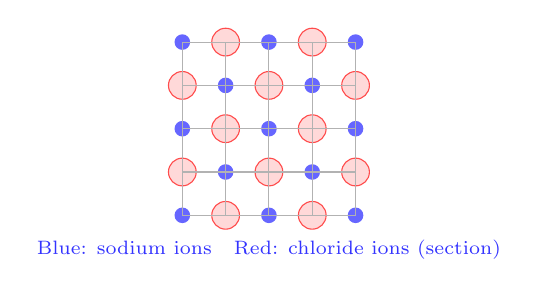
\begin{tikzpicture}[scale=0.55]
\foreach \x in {0,1,2,3,4}
  \foreach \y in {0,1,2,3,4} {
    \pgfmathparse{mod(\x+\y,2)}
    \pgfmathtruncatemacro{\parity}{\pgfmathresult}
    \ifnum\parity=0
      \fill[blue!60] (\x,\y) circle (0.18);
    \else
      \draw[red!70,fill=red!15] (\x,\y) circle (0.32);
    \fi
  }
\draw[gray!60] (0,0) grid (4,4);
\node[blue!80] at (2,-0.8) {\scriptsize Blue: sodium ions\quad Red: chloride ions (section)};
\end{tikzpicture}
\end{center}

This is a schematic cross section. Circle sizes and colors are conventions, and ions are not solid balls. Actual chloride ions are nearly twice as large as sodium ions (Chapter 11 measured their ``waistlines''). There is just one key message: \textbf{opposite signs sit next to each other; like signs face across them, filling an alternating array}.

A salt grain therefore contains no ``sodium chloride molecules.'' No particular pair is closer than the others or forms its own household; every ion belongs to the whole city. To exaggerate a little, \textbf{an entire salt grain is one ``molecule''}: a city of ions held together by electrostatic attraction.

How big is this city? Consider a grain with 1-millimeter sides, a volume of about 1 cubic millimeter. Salt's density is about \ud{2.16}{g/cm^{3}}, giving a mass of about $2.2\times 10^{-3}$ grams. Sodium chloride's molar mass is about \ud{58.4}{g/mol}, so this is $3.7\times 10^{-5}$ moles. Multiplying by Avogadro's constant, \ud{6.02\times 10^{23}}{mol^{-1}}, gives about $2.2\times 10^{19}$ ``sodium--chloride units,'' or over $4\times 10^{19}$ ions. A tiny pinch of salt contains more ions than a billion for every person on Earth.

\section{The Rules: Electrostatic Accounting}

The force holding this city together is familiar: the same electrostatic force that lets a rubbed balloon lift your hair. Its rule is Coulomb's law: the force between two charged particles is proportional to the product of their charges and inversely proportional to the square of their separation. Opposite charges attract; like charges repel.

This rule, together with ``ions avoid neighbors of the same sign,'' explains all of salt's quirks at once:

\textbf{Why hard, and why a high melting point?} Melting requires ions to escape their neighbors' attractions in every direction and begin sliding freely. Any one nearest-neighbor attraction is unremarkable, but each ion has 6 nearest neighbors, then next-nearest neighbors, and so on. Together, the whole city holds a huge ``cohesion deposit.'' Separating 1 mole of salt crystals into widely separated gaseous ions requires about \ud{787}{kJ/mol}. This is the \textbf{lattice energy}, a measure of how firmly an ionic crystal holds together. A large lattice energy means a high melting point: salt melts only at $801\,^{\circ}\mathrm{C}$, whereas sugar molecules lack this electrostatic cement and fall apart above a hundred degrees Celsius.

\begin{qiaoliang}
Now we can settle the complete energy account for sodium meeting chlorine (per mole):
\begin{itemize}[itemsep=1pt]
\item Sodium gives up an electron: $+496$ (ionization energy, an expense).
\item Chlorine accepts it: $-349$ (electron affinity, a return).
\item Gas-phase subtotal: $+147$---\textbf{a loss}.
\item Ions assemble into a crystal: $-787$ (lattice energy, a large profit).
\end{itemize}
Total: $+147-787=-640$ (kJ/mol), a major energy reduction, so the deal goes through. Notice two things. First, the driving force is not ``chlorine wanting eight electrons''---atoms have no wishes---but the \textbf{whole city's} much lower energy than the separated atoms. Second, the first two terms alone make a one-to-one gas-phase reaction unprofitable; lattice energy's ``city-building dividend'' turns the entire balance around. This is why ionic bonds always appear in crystals rather than isolated ion pairs.
\end{qiaoliang}

\textbf{Why brittle?} Hardness and brittleness often occur together, but deserve separate explanations. Salt is hard because electrostatic attraction is strong, and brittle because that attraction is very particular about arrangement. Imagine sliding the upper half of a crystal half a lattice spacing along a plane. Previously opposite-sign neighbors now face ions of the same sign. Attraction instantly flips to repulsion, and crack!---the crystal splits cleanly along that plane. These are the neat fracture faces you see when crushing salt. Metals deform under a hammer instead of shattering because they use a completely different kind of bonding (Chapter 21).

\textbf{Why are some ionic crystals even tougher?} Coulomb's law has two controls: charge and distance. Larger charges and smaller ions (closer packing) mean stronger attraction and higher lattice energy. Compare salt's $+1$ and $-1$ ions and $801\,^{\circ}\mathrm{C}$ melting point with magnesium oxide's smaller $+2$ and $-2$ ions. Its lattice energy is about five times salt's, and its melting point reaches $2852\,^{\circ}\mathrm{C}$---high enough for refractory bricks in steelmaking furnaces. Charge density (charge packed into a unit volume) is a useful guide to an ionic crystal's personality.

\section{Symbols: NaCl Is a Recipe, Not a Molecule}

Only now do the symbols formally enter, because you know what they should and should not say.

The sodium--chlorine reaction is written:
\[\chem{2Na} + \chem{Cl_2} \rightarrow \chem{2NaCl}\]
The \chem{NaCl} in the two product units is read ``sodium chloride,'' but it is only an \textbf{empirical formula}. It promises that ``this crystal has sodium and chloride ions in a $1:1$ ratio,'' not that any ``\chem{NaCl} molecules'' exist. Like saying ``this city has a $1:1$ ratio of men to women,'' it is a population statistic, not a claim that everyone is locked into a pair.

The same logic gives other ionic compounds' recipes. In \chem{MgCl_2}, magnesium ions carry $+2$ and chloride ions $-1$, so one magnesium accompanies two chlorides and the charges cancel exactly. In \chem{Na_2O}, two sodium ions accompany one oxide ion. An ionic crystal's formula is essentially a \textbf{charge-balance sheet}: count each ion's charge, then find the smallest ratio that balances positives and negatives. The \chem{CO_3^{2-}} in calcium carbonate, \chem{CaCO_3}, is a ``polyatomic ion,'' several atoms grouped together. Internally, another kind of bond joins them (Chapter 19's covalent bond), but externally the group behaves as a single ion with charge $-2$, lining up in the city like the others.

Only in unusual settings such as salt vapor do short-lived isolated pairs of ``one sodium ion plus one chloride ion'' exist. Those can just about be called ``\chem{NaCl} molecules,'' but you will practically never encounter them.

\section{Evidence: X-Rays ``Saw'' the Lattice}

\begin{zhengju}
The conclusion that ``salt contains no molecules'' was not a clever guess; a beam of X-rays forced scientists to accept it.

The story begins in 1912. The German physicist Laue was pondering a question about waves. X-rays had been discovered only a little over a decade earlier, and nobody was certain they were waves. Laue reasoned that if X-rays were very short-wavelength waves, and crystals really contained regularly arranged atomic lattices, X-rays passing through a crystal should diffract like light passing through a fine grating, producing regular spots on a photographic plate. The experiment produced exactly such an orderly pattern, answering two questions at once: X-rays were waves, and crystals were lattices.

The next year, Britain's Braggs---father William Henry and son Lawrence---turned this effect into a ``ruler for internal crystal spacings.'' The positions and angles of diffraction spots reveal distances between neighboring particles. Salt was among their first samples.

The result made chemists uncomfortable. They had expected especially close pairs of ``sodium chloride molecules'': one sodium with one chlorine, like partners at a dance. Instead, the data were clear: only one arrangement existed, with sodium and chlorine alternating at uniform separations and no two particles ``especially close.'' \textbf{The expected molecular pairs simply did not exist.} The elder Bragg initially resisted and tried other arrangements, but only the ``alternating ion array'' predicted spot positions matching the plates exactly. Evidence overruled habit, and chemists had to accept that salt contained no salt molecules.

The method also measured ionic ``waistlines,'' confirming another counterintuitive fact: sodium ions were almost half the size of sodium atoms, while chloride ions were larger than chlorine atoms, agreeing with Chapter 11's periodic reasoning. In 1915, father and son shared the Nobel Prize in Physics. Lawrence was 25 and remains among the youngest recipients of a scientific Nobel Prize. The methodological lesson is worth remembering: they had no photograph directly showing ions, only spots. Repeatedly and carefully working backward from ``if the arrangement is this, the spots should be there'' turned an invisible lattice into accepted evidence.
\end{zhengju}

\section{Conductivity: Charge Must Be Free to Move}

Return to our third opening guess. Dry salt clearly consists of charged particles, so why does it not conduct?

The answer lies in an easily missed distinction: conduction requires not ``the presence of charge,'' but ``\textbf{charge that can move}.'' Current is the directed movement of charge. In solid salt, neighbors' attractions lock each ion to a lattice site, leaving it only able to shiver in place (thermal vibration). Full of charge but unable to move, it is naturally an insulator.

Two methods ``release'' the ions. Heating until melting breaks up the lattice into a liquid, allowing ions to roam. Dissolving in water lets water molecules invite ions down from the city walls one by one (Chapter 23 explains how), leaving them swimming freely. Connect either state to a power supply and positive ions head toward the negative electrode while negative ions head toward the positive one. These oppositely directed ion streams form a current. This differs from conduction in metals: there, electrons move (Chapter 21); in salt solution, entire ions move.

\textbf{Translator safety note:} Do not carry out the saltwater electrolysis activity below at home. Its bubbles need not be only products of water decomposition: chloride electrolysis can produce chlorine-containing chemicals. Never smell or collect the gas, and never short the battery by touching electrodes together. Use a teacher-selected, risk-assessed demonstration instead. See \href{https://www.acs.org/molecule-of-the-week/archive/s/sodium-hypochlorite.html}{ACS on salt-solution electrolysis} and \href{https://www.cdc.gov/chemical-emergencies/chemical-fact-sheets/chlorine.html}{CDC chlorine guidance}.

\begin{shiyan}
\textbf{A Three-Cup Conductivity Test}

Materials: a 9V battery (or two AA batteries and a holder), a small buzzer (or an LED in series with an approximately 220-ohm resistor), three or four leads with crocodile clips, table salt, white sugar, purified water, three clean cups, and two graphite electrodes (sharpened pencil leads can substitute).

Procedure: (1) Connect the battery, buzzer, and two electrodes in series. Briefly touch the electrodes together to check that the buzzer sounds and the circuit works. (2) Insert the electrodes into a pile of dry salt without letting them touch. Does it buzz? (3) Dissolve the salt in half a cup of purified water and insert the electrodes again, still apart. What happens now? (4) Repeat with a sugar solution of the same concentration. (5) You can also look closely at the electrode surfaces: tiny bubbles often appear in saltwater as the current decomposes water. (Chapter 12's sodium is ``electrolyzed'' from molten salt in this way, except industry uses high-temperature molten salt.)

What to observe: dry salt gives no buzz, saltwater does, and sugar water essentially does not. Solid salt locks up its ions, while water sets them free. Dissolved sugar remains molecular and produces no charges that can move.

Safety note: use batteries only; \textbf{never use electricity from a wall outlet}. Do not let the electrodes touch directly (a short circuit can overheat the battery). Pencil leads become brittle after soaking; discard them afterward. Wash all equipment after the experiment and never taste any experimental material.
\end{shiyan}

This property, ``conducting only once released,'' is more than a kitchen curiosity; it underpins a major industry. Heat salt until molten and pass a strong current through it, and ions are forced toward opposite electrodes, giving up or taking back electrons. Silvery sodium metal forms at the cathode, and yellow-green chlorine bubbles from the anode. Chapter 12's water-reactive sodium is ``electrolyzed'' from quiet white salt this way. Electrolyzing aqueous salt solution (the chlor-alkali industry) produces caustic soda, chlorine, and hydrogen together, supplying raw materials for fertilizers, plastics, disinfectants, and papermaking. The same freely moving ions also explain why physiological saline can be used in hospital infusions, why seawater conducts, and why electrical signals travel through nerve cells. They will return repeatedly when we discuss life.

\section{Some Salts Dissolve; Others Refuse to Budge}

One question remains. All are ionic crystals, yet table salt dissolves on contact with water, while eggshells and limestone (mainly calcium carbonate) can soak for years with no visible loss. The ``barium meal'' (barium sulfate) swallowed for digestive-tract imaging is even more insoluble. Why the difference?

Dissolving is a tug-of-war. On one side stands lattice energy: removing ions from the city walls incurs a ``demolition fee,'' greater for a more firmly bonded city. On the other stands water: water molecules surround and accommodate the removed ions, releasing a ``settling-in allowance'' (heat of hydration). When the allowance exceeds the demolition fee, dissolution proceeds readily; when demolition costs too much, the crystal stays put. Salt's ions carry small charges and its lattice energy is moderate, so water can afford the allowance and salt dissolves readily (about 36 grams per 100 grams of water at $25\,^{\circ}\mathrm{C}$). Calcium carbonate has $+2$ against $-2$, sharply raising lattice energy beyond water's means; only a dozen or so milligrams dissolve per liter. Chapters 23 and 25 will settle the details---why water surrounds ions and how temperature and pressure interfere. For now, establish the framework: \textbf{solubility is the energy balance between ``dismantling the lattice'' and ``settling the ions.''}

This balance can both save and harm lives. Barium ions, \chem{Ba^{2+}}, are toxic, and soluble barium chloride can be fatal. But barium sulfate is so insoluble that swallowing it releases almost no barium ions. It passes through the intestine unabsorbed and blocks X-rays, making it useful as a contrast agent that lets doctors see the digestive tract's outline. Whether the same element is a poison or a diagnostic tool depends entirely on the crystal imprisoning it. This is another lesson in ``dose, form, and evidence'': discussing whether an element is toxic without specifying its compound is meaningless.

Winter deicing salts (often calcium chloride) use the same principles: heat released as calcium chloride dissolves helps melt snow, while the dissolved ions also interfere with freezing. Chapter 25's discussion of solution properties will revisit that account.

\section{Boundaries: Perfectly Ionic Bonds Do Not Exist}

Our model---complete electron transfer and an orderly array of charged-ball-like ions---works very well for combinations with large electronegativity differences, such as salt and magnesium oxide. But it has a clear boundary. A small, highly charged positive ion strongly pulls the diffuse electron cloud of a large negative ion toward itself. Electrons are no longer ``fully transferred,'' but ``very unevenly shared.'' Such crystals begin behaving unlike typical ionic crystals. Aluminum chloride, for example, has a low melting point and readily sublimes on heating, behaving more like a molecular substance.

In other words, \textbf{ionic and covalent bonds are not separate rooms, but opposite ends of a continuous spectrum}. Chapter 11's electronegativity difference roughly locates a bond on that spectrum: a larger difference puts it nearer the ionic end, a smaller difference nearer the sharing end. Salt sits at the ionic extreme, making this chapter's story neat and clear, but most bonds lie somewhere in between.

\begin{wuqu}
Misconception: ``When salt dissolves, water washes individual sodium chloride molecules apart.''

There are two counterexamples. First, this chapter's X-ray evidence: solid salt has no ``sodium chloride molecules'' in the first place, only an alternating ion array, so no molecules can be washed apart. Second, heat salt until it melts without adding any water: molten salt still conducts, showing that ions can move freely and exist independently once released from the lattice. Dissolving does not ``dismantle molecules,'' but ``dismantles the lattice.'' Water invites ions off the walls, surrounds them separately, and carries them away. This is not pedantry: it determines why saltwater conducts but sugar water does not, and why the ``salt'' in your body never works as ``molecules.''
\end{wuqu}

\section{Back to the Salt Grain}

Now let us fulfill our opening promises.

Why is salt square? Because its internal ion lattice is itself a cubic grid. The crystal's exterior is a macroscopic portrait of its internal arrangement: countless ions lined up in cubic ranks naturally build a square-edged object. It remains square when crushed because blows split it along weak crystal planes where like-sign ions face each other, leaving smaller cubic arrays.

Why does it fear water but not fire? Water can afford the settling-in allowance, removing ions from the walls one by one. Fire must pay the huge lattice energy to dismantle the whole city, and an ordinary flame falls far short: melting requires $801\,^{\circ}\mathrm{C}$.

Why does dry salt insulate while saltwater conducts? The key is never ``whether charges exist,'' but ``whether they can move.'' Electrostatic forces lock solid-state ions to lattice sites; entering water restores their freedom.

An ordinary salt grain thus links particles, rules, symbols, and evidence into one complete chain---exactly the path this book has been following.

\section{Must Electrons Be Transferred Outright?}

Sodium and chlorine's story is decisive because their abilities differ so greatly: one cannot hold on, the other grabs fiercely, and the electron changes ownership outright. Most atomic encounters involve no such mismatch. Hydrogen meets chlorine, carbon meets oxygen, oxygen meets hydrogen: neither partner can completely steal the other's electron, so the standoff ends in \textbf{sharing}.

How do shared electrons bind atoms together? Why does sharing produce ``real molecules,'' with definite shapes and independent identities, able to change from water to vapor and back? What happens if the sharing is unequal? These answers open the gateway to organic molecules, water, and life. Next comes Chapter 19: covalent bonding.

\begin{tiaozhan}
Why is lattice energy so much larger than ``one ion pair's attraction''? List the accounts term by term: each ion attracts 6 nearest neighbors of opposite sign, repels 12 next-nearest neighbors of like sign, then encounters 8 opposite-sign ions, 6 like-sign ions, and so on, alternating in sign and decreasing with distance squared. Adding infinitely many terms converges mathematically to a pure number, about $1.748$ for the salt structure, called the \textbf{Madelung constant}. It means each ion in a crystal enjoys a net electrostatic attraction about $1.75$ times that of an isolated ion pair. A city really is cheaper than a world of two, and the savings can be calculated precisely. Multiply Coulomb's law by the Madelung constant and add a correction for repulsion when electron clouds get too close, and you can calculate salt's lattice energy from scratch, agreeing within a few percent with the experimental \ud{787}{kJ/mol}. This is the strongest quantitative success of the ``ionic bonding is electrostatics'' model. Drawing every step in this chapter's accounts (sublimation, ionization, electron affinity, and bonding) as an energy cycle gives physical chemistry's famous ``Born--Haber cycle.'' You can skip this box without losing the main thread, but it provides an entry point if you wonder how Coulomb's law can explain an entire crystal.
\end{tiaozhan}

\section*{Try It}

\begin{sikaoti}
\item Draw a $4\times4$ two-dimensional ion array like this chapter's diagram. Choose a positive ion, circle its nearest opposite- and like-sign neighbors, and use arrows to show attraction and repulsion. Explain why the crystal neither falls apart nor collapses into a clump.
\item Draw an energy-step diagram with reaction progress horizontally and energy vertically. Show ``sodium ionization $+496$,'' ``chlorine accepts an electron $-349$,'' and ``ions form a crystal $-787$'' (in kJ/mol), marking the net change. Would a metal with an exceptionally high ionization energy readily form ionic crystals? Why?
\item Without looking anything up, use the two controls ``charge'' and ``ionic radius'' to predict whether magnesium oxide, \chem{MgO}, melts above or below salt, explaining why. Then predict which melts higher, magnesium oxide or calcium oxide, \chem{CaO} (calcium ions are larger than magnesium ions). Check your reasoning against published data.
\item Two unlabeled cups hold clear liquids: concentrated saltwater and concentrated sugar water. Design a way to distinguish them using this chapter's experimental equipment, stating the principle. Then consider: if a liquid conducts, does that prove its solute must be an ionic crystal when solid? (Hint: acetic acid is molecular, yet its aqueous solution conducts because it produces ions ``on site'' in water. Chapter 26 explains.)
\item Calcium carbonate is poorly soluble in water, yet eggshells slowly dissolve and bubble in vinegar. Using ``lattice demolition cost versus water's settling-in allowance,'' propose which side vinegar helps and how. (Hint: the bubbles are carbon dioxide escaping the solution.)
\item This chapter estimated about $4\times10^{19}$ ions in a salt grain with 1-millimeter sides. If lined up side by side, each occupying about $0.3$ nanometers, how long would the line be? Compare it with the Earth--Moon distance, about 380,000 kilometers.
\end{sikaoti}
